%\part{Results}

\chapter{Results}
\section{Sensitivity analysis}
TODO
This clustering analysis was conducted on $n=100$ observations, the former 50 of which were iid sampled from a $\Nc(4,1)$ and the latter from a $\Nc(7,1)$.
We chose the prior parameters for the Normal-NIG model (\ref{nnig}) as follows: $\mu_0 = 5, \lambda_0 = 1, \alpha_0 = 2, \beta_0 = 2$.
The \verb|Neal8| algorithm with $m=3$ auxiliary blocks was run for 20000 iterations, and the first 5000 were discarded as burn-in, for a total of $K=15000$ valid iterations.
We will keep these parameters values fixed unless explicitly stated. \\
The following test data were all saved to \verb|.csv| files and used for the realization of plots with the \verb|ggplot2| R package.

\subsection{Oscillations}
After running the algorithm as described above with total mass $M=0.25$, we find that the obtained clusterings and local density estimates are highly fluctuating over the iterations of the algorithm, as shown in figure \ref{fig:fluctuations}:
\begin{figure}[h]
	\centering
	\begin{minipage}{0.5\textwidth}
		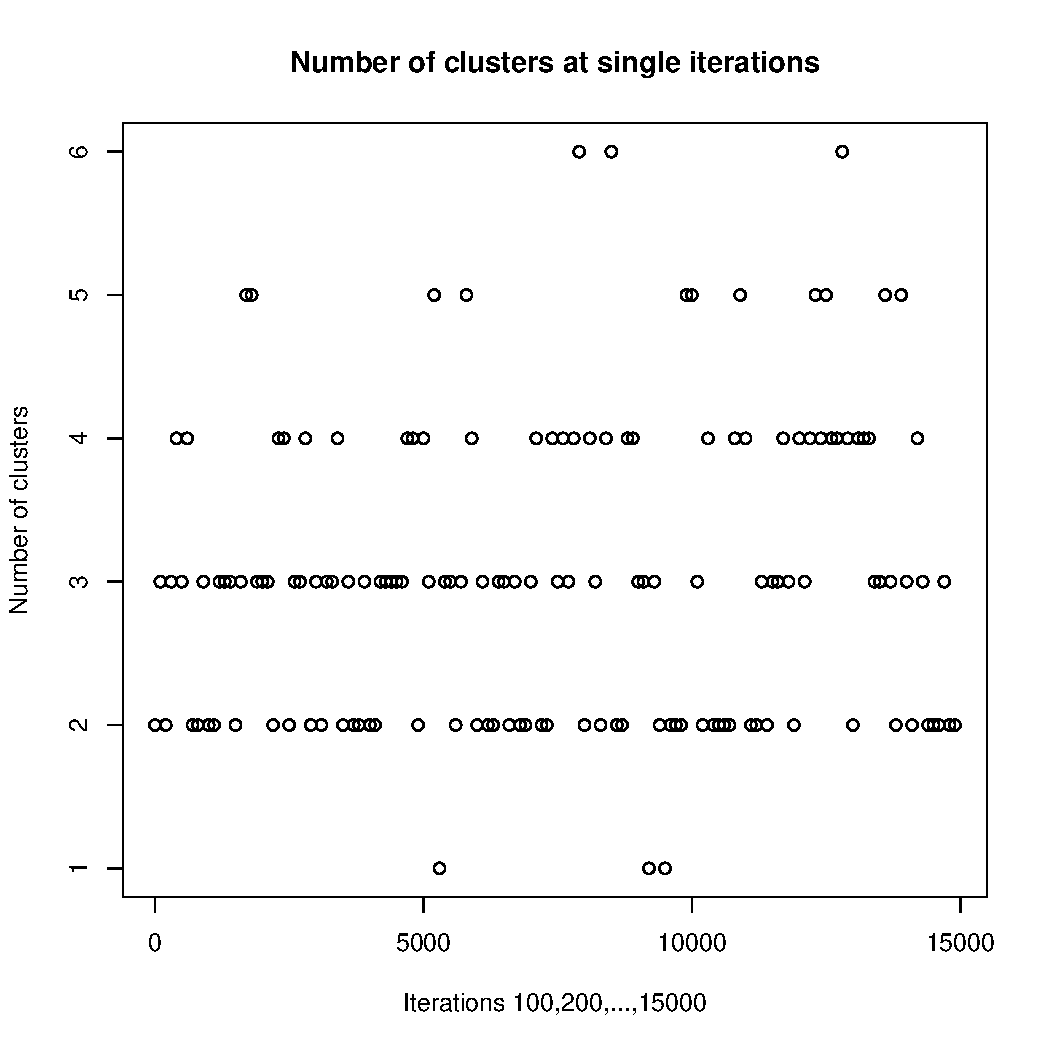
\includegraphics[scale=0.35]{etc/cardinalities_thinned.pdf}
	\end{minipage}%
	\begin{minipage}{0.5\textwidth}
		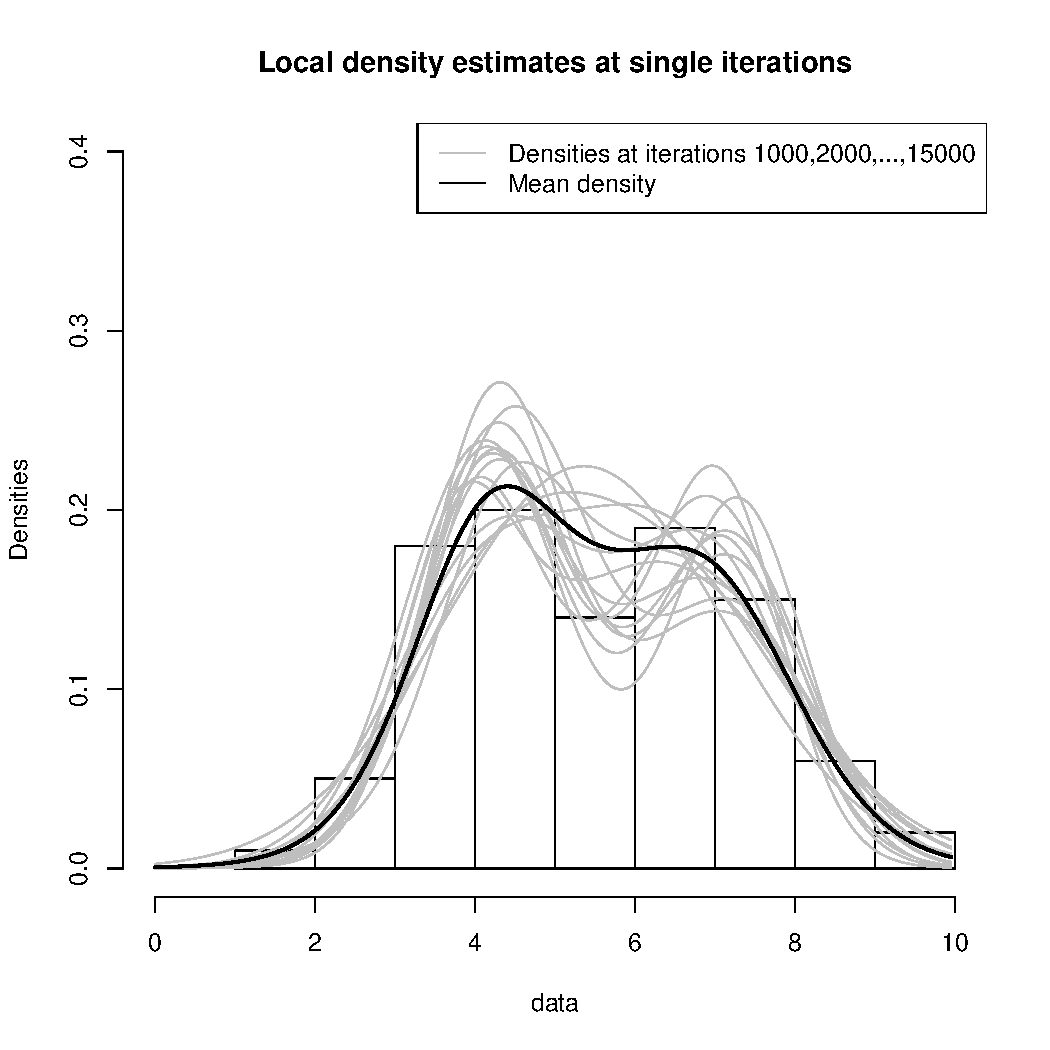
\includegraphics[scale=0.35]{etc/densities_iters.pdf}
	\end{minipage}
	\caption{Clustering and density fluctuations over iterations}

	\label{fig:fluctuations}

\end{figure}

In both plots, a thinning of one iteration every 100 and every 2500, respectively, was performed for better readability of the plot.
In the right side plot, the local densities are compared with the histogram of the data as well as the final estimate provided by the mean density.
We can see that the number of clusters at all iterations varies significantly between 1 and 6, even in the last thousands of iterations, and the same behavior applies to the local density estimates. 
This is further confirmation of the fact that the single iterations themselves do not converge.
Instead, as previously discussed, the convergence is in the \emph{mean}, both for the density estimate and for the average dissimilarity matrix which we use to find the best clustering.

\subsection{Total mass}
Let us now examine the role of the total mass parameter, $M$.
We ran the algorithm with several values for $M$ whilst keeping the other parameters unchanged from the ones indicated at the beginning of the section.
For each $M$, we saved the number of clusters of the best clustering produced by the algorithm, and studied the overall behavior varying $M$, shown in figure \ref{fig:n_clusters_M}.

\begin{figure}[h]
	\centering
	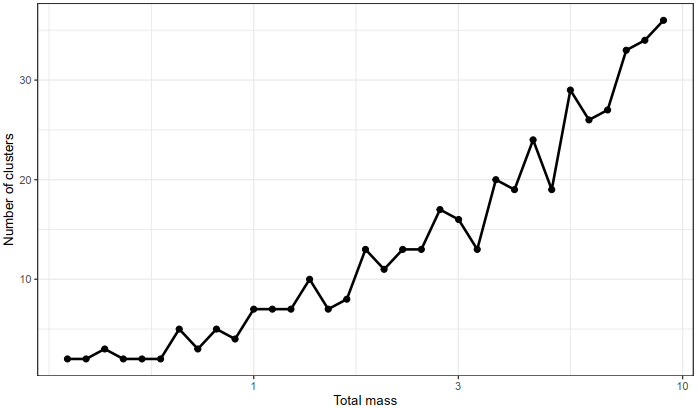
\includegraphics[scale=0.5]{etc/clusters.PNG}
	\caption{Number of clusters as a function of the total mass}

	\label{fig:n_clusters_M}

\end{figure}

Note that the values for $M$ were chosen so as to be evenly spaced in log-scale, thus the abscissa is in log-scale as well.
We can note that the clusters are increasing with the total mass.
This is consistent with the fact that the probability of creating a new cluster is proportional to $M$, as seen in (\ref{neal8prob}). \\
Moreover, we can see in figure \ref{fig:density_M} the density estimates for some of the values of $M$ (again, compared with the histogram of the data).

\clearpage

\begin{figure}[h]
	\centering
	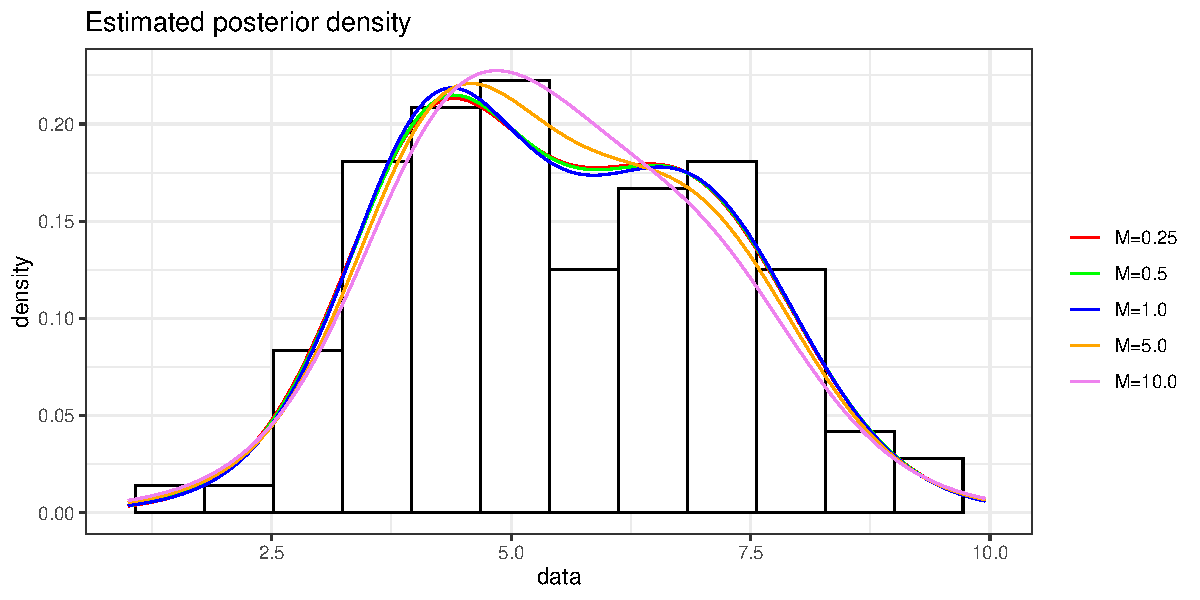
\includegraphics[scale=0.55]{etc/dens_withMm3.pdf}
	\caption{Density estimates varying the total mass}

	\label{fig:density_total_mass}
\end{figure}


In our case, lower values for the total mass account better for the distribution of the data points, with the modes being near the real expected values of the two normal distributions, 4 and 7.
On the other hand, higher values tend to clump together all 100 observations as though they were extracted from a single distribution.
As we can see, the total mass $M$ acts as smoothing parameter and, given its strong influence on the number of mixture components, it is a prime candidate for a prior distribution being put onto it.



\subsection{Auxiliary blocks}
We shall now try and change the number of auxiliary blocks $m$, and check how this impacts the density estimation.
For this test, a large total mass $M=10$ was chosen; the reason being that a small $M$ would not allow significant differences as $m$ changes.
Indeed, $m$ directly influences only the estimate (\ref{margneal8}) of the marginal distribution, that has a weight of $\frac{M}{M+n}$ (as seen in (\ref{localdens})), which is negligible if $M$ is small.
Therefore, $M=10$ was picked, and the result is displayed in figure \ref{fig:density_n_aux}.


\begin{figure}[h]
	\centering
	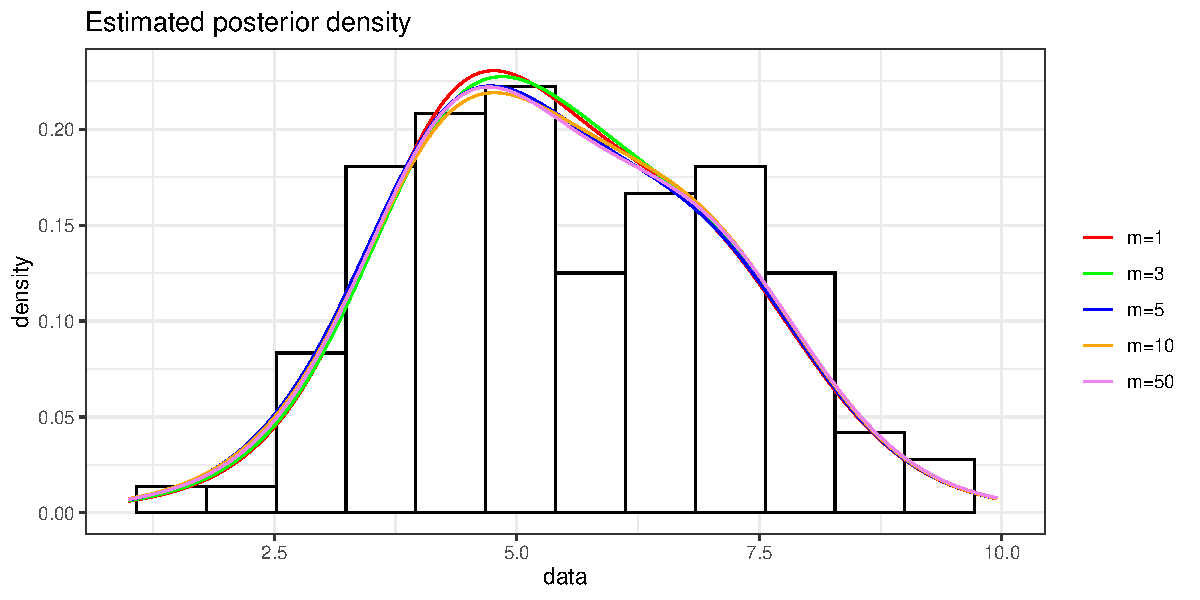
\includegraphics[scale=0.55]{etc/dens_withmM10.pdf}
	\caption{Density estimates varying the number of auxiliary blocks}

	\label{fig:density_n_aux}
\end{figure}

Note that a larger $m$ gives a better estimate of the marginal, because the sample mean is computed over a larger number of terms and the algorithm approximates the behavior of the algorithm \verb|Neal2|.



\subsection{Density components}
We now wish to visualize how the local density is computed at a given sample iteration.
Let us run again the \verb|Neal8| algorithm with both $M=0.25$ and $m=3$ fixed, and then use the \verb|cluster_estimate()| function to extract the best clustering for the data.
We find that it is at iteration 2490, which gives 2 clusters.
As shown in \ref{localdens}, each of these clusters has its own density estimate, which we refer to as \emph{component}, and a weight attached to it proportional to its cardinality.
The weighted sum of these components gives the ``full'' local estimate of the density for that iteration.
The plot in figure \ref{fig:components_density} shows both the \emph{weighted} components and their sum.
\begin{figure}[h]
	\centering
	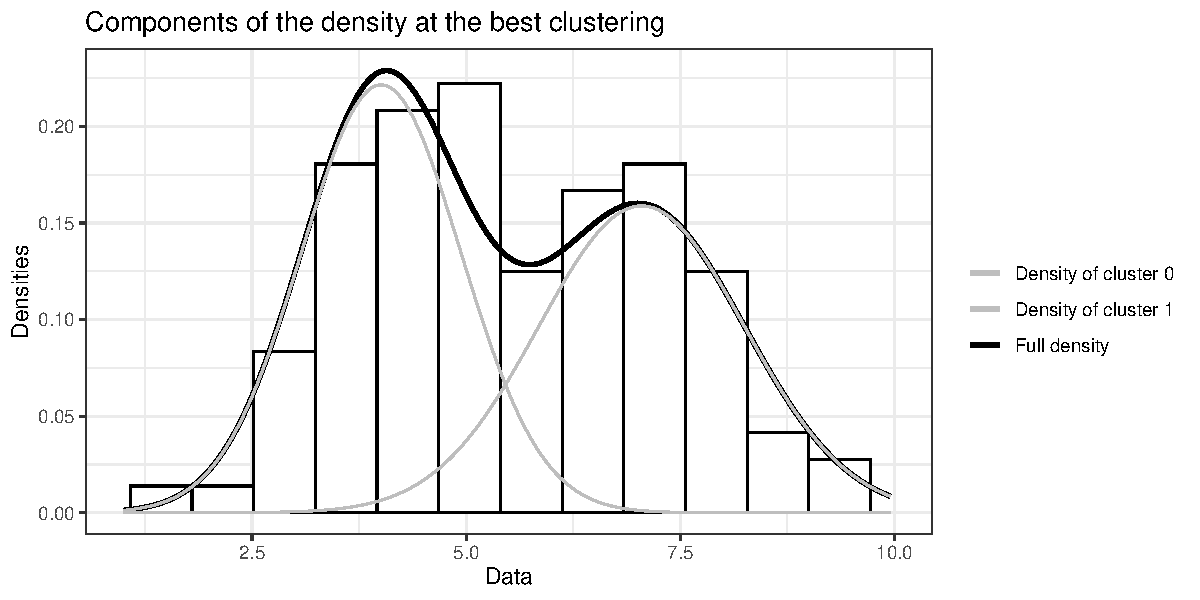
\includegraphics[scale=0.6]{etc/componentsM025m3_best.pdf}
	\caption{Weighted components and full density estimates}

	\label{fig:components_density}
\end{figure}

In this case the weights turn out to be approximately equal (0.52 and 0.48 respectively).
Again, the two components are concentrated around the true means (4 and 7) of the likelihoods of the data points, as expected. \\
In other cases, the best clustering may produce more than 2 clusters.
One such example is given by the best clustering of \verb|Neal8| run with $M=1$ (and $m=3$ as before), found at iteration 6611.
Although there are 7 clusters, all weights bar the first two are insignificant, as we can see in figure \ref{fig:cluster_weigths}, making the corresponding components have almost zero impact in the weighted sum of the local estimate.

\clearpage

\begin{figure}[h]
	\centering
	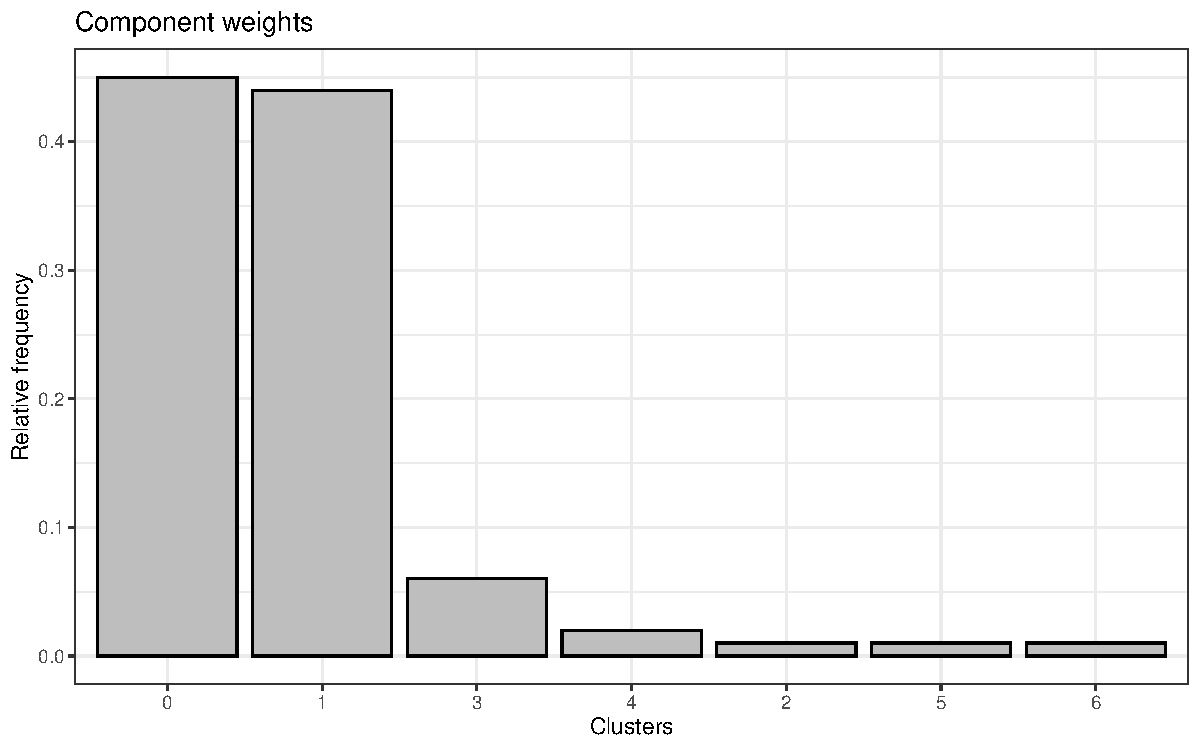
\includegraphics[scale=0.4]{etc/barplotM1m3.pdf}
	\caption{Clusters weights}

	\label{fig:cluster_weigths}
	
\end{figure}



\subsection{\texttt{Neal2} vs \texttt{Neal8}}
Finally, we ran the \verb|Neal2| algorithm with the same parameters as \verb|Neal8| (indicated at the beginning of the section) as well as $M=10$ for both.
Again, a rather large total mass was chosen in order to better highlight the difference in the marginal estimate.
In fact, in the \verb|Neal2| case, since the marginal distribution is known in closed form, the estimate is more accurate. A qualitative analysis is shown in figure \ref{fig:neal2_neal8}.

\begin{figure}[h]
	\centering
	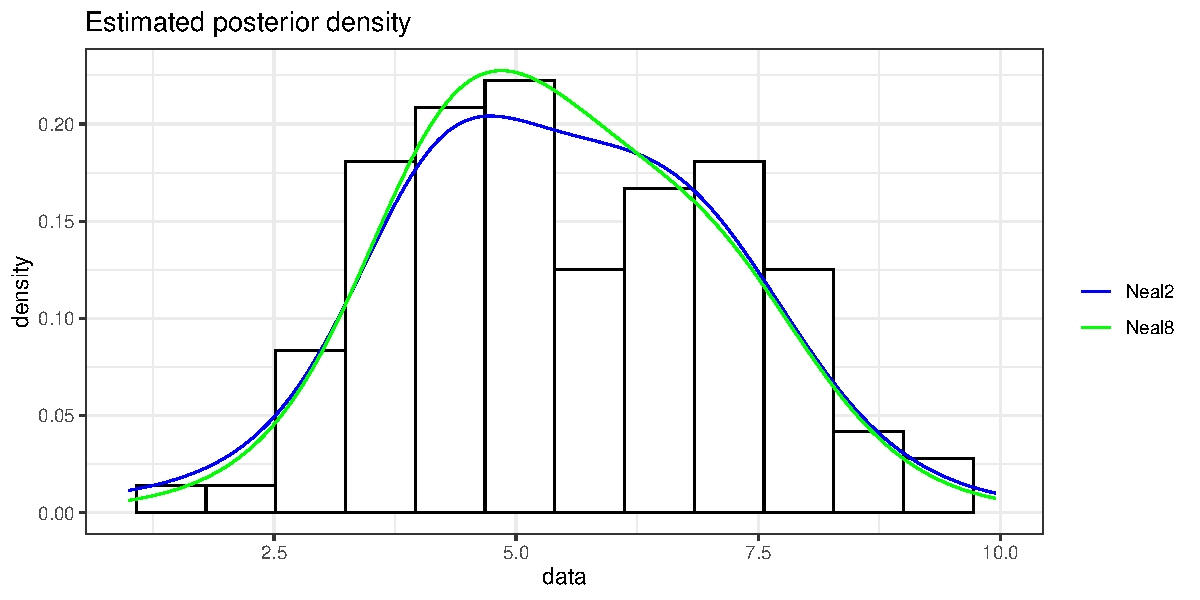
\includegraphics[scale=0.55]{etc/neal2_M10.pdf}
	\caption{Neal2 and Neal8 density estimates}

	\label{fig:neal2_neal8}
\end{figure}
